\documentclass[12pt]{beamer}

\usetheme{TCT}
\usecolortheme{dolphin}

\usepackage[normalem]{ulem}
\usepackage{color}
\usepackage[utf8]{inputenc}
\usepackage[IL2]{fontenc}

\usepackage{amsmath}
\usepackage{graphicx,xcolor}
\usepackage{amsthm}
\usepackage{mathtools}
\usepackage{amsfonts}

\usepackage{hyperref}

\newcommand{\at}{\makeatletter @\makeatother}

%\useinnertheme{circles}

\title{\textbf{Twitter Crowd Translation}}
\author{
\underline{Eduard \v{S}ubert} %\\
%Faculty of Nuclear Sciences and Physical Engineering\\
%Czech Technical University in Prague\\
%\and
and
{Ond\v{r}ej Bojar}\\
%Institute of Formal and Applied Linguistics\\
%Faculty of Mathematics and Physics\\
%Charles University, Prague, Czech Republic
}

\begin{document}

% It goes without saying that social networks have gained tremendous popularity. In my presentation I will assume that everyone here is familiar with the concept of social networks.
\setbeamercolor{background canvas}{bg=TCTwhite}
\frame{\titlepage}


% To get a better picture of the situation let's look at Twitter statistics, these are really impressive numbers. So let's look at one more.
\setbeamercolor{background canvas}{bg=TCTblue}
\setbeamercolor{normal text}{fg = TCTsilver}
\setbeamercolor{frametitle}{fg = TCTwhite}
\begin{frame}
	\frametitle{Twitter Usage}
	\vfill
	\begin{center}
	\textcolor{TCTsilver}{\Large 284 million monthly active users}
	\\[0.7cm]
	\textcolor{TCTsilver}{\Large 500 million Tweets are sent per day}
	\\[0.7cm]
	\textcolor{TCTsilver}{\Large 80\% of Twitter active users are on mobile}
	\end{center}
	\vfill
	\hfill\textcolor{TCTsilver}{https://about.twitter.com/company}
\end{frame}

% At first it seem impressive.
% But it is of course support only for the interface not for the content
% So if I decide to tweet in English my mother who only speak Czech won't be able to read my tweets; which might be a good thing
% But are other situations like the one in Ukraine. Here we may wish for all the tweets concerning the topic to reach great audience without the language barrier
% and that is precisely what we decided to do
\setbeamercolor{background canvas}{bg=TCTsilver}
\setbeamercolor{normal text}{fg = TCTsilver}
\setbeamercolor{frametitle}{fg = TCTgray}
\begin{frame}
	\frametitle{Twitter Usage}
	\vfill
	\begin{center}
	\textcolor{TCTgray}{\Large Twitter supports 35+ languages}
	\end{center}
	\vfill
	\hfill\textcolor{TCTgray}{https://about.twitter.com/company}
\end{frame}

% So what goals do we have? Broadly we want to provide translations of tweets. 
% Of course we want to be accurate, fast and we don't want to force users to visit our website to access translations or something like that
% In ideal world we would deploy a machine translator and be done with it. But if you have ever tried to understand machine translated tweet
% you know that is not the way to go. If you did not, let me show you an example

\setbeamercolor{background canvas}{bg=TCTblue}
\setbeamercolor{normal text}{fg = TCTsilver}
\setbeamercolor{frametitle}{fg = TCTwhite}
\begin{frame}
	\frametitle{Goals}
	\begin{itemize}
		\item \textcolor{TCTsilver}{provide translations of tweets}
		\item \textcolor{TCTsilver}{accurate}
		\item \textcolor{TCTsilver}{fast (aiming at ``instant'')}
		\item \textcolor{TCTsilver}{stay within the Twitter platform}
	\end{itemize}
\end{frame}

% In the spirit of recent success of comet harpooning here is a tweet from the lander translated by the Moses MT from original English to Czech and back to English. 
% It is of course not really usable. I would like to point out that the second English translation is actually better representation of the original tweet then the Czech translation in the middle.
% There needs to be work done on preprocessing for example to better deal with the hashtags but we find the lack of appropriate training data to be the main issue.
\setbeamercolor{background canvas}{bg=TCTsilver}
\setbeamercolor{normal text}{fg = TCTsilver}
\setbeamercolor{frametitle}{fg = TCTgray}
\begin{frame}
	\frametitle{Machine Translated Tweet}
	\begin{center}
	\textcolor{TCTgray}{\Large @Philae2014:}
	\\[0.5cm]
	\textcolor{TCTblue}{Some problems with my cold gas thruster could mean that it might be up to harpoons \& ice screws to make sure I stay on \#67P  \#CometLanding}
	\\[0.5cm]
	\textcolor{TCTgray}{některé problémy se zimou plynových trysek by mohlo znamenat, že by to mohlo být až harpuny \& mnaga; led šrouby, aby se ujistil, že zůstane na 67 P \# \# cometlanding }
	\\[0.5cm]
	\textcolor{TCTblue}{some problems with cold gas jets could it be to harpoon \& mnaga; ice screws to assure that stays on 67 p \# \# cometlanding }
	\end{center}
\end{frame}

% Therefore we have added additional goal. To collect human translated parallel corpus.
% This is the point where the TCT comes to be. It is a system for human translation and evaluation of twitter posts; tweets.
\setbeamercolor{background canvas}{bg=TCTblue}
\setbeamercolor{normal text}{fg = TCTsilver}
\setbeamercolor{frametitle}{fg = TCTwhite}
\begin{frame}
	\frametitle{Goals}
	\begin{itemize}
		\item \textcolor{TCTsilver}{\Large collect appropriate parallel corpus}
		\item \textcolor{TCTsilver}{provide translations of tweets}
		\item \textcolor{TCTsilver}{accurate}
		\item \textcolor{TCTsilver}{fast (aiming at ``instant'')}
		\item \textcolor{TCTsilver}{stay within the Twitter platform}
	\end{itemize}
\end{frame}

% TCT of course autonomously collects tweets for translation and publishes the translated results.
% Let's now look at the design in more detail.
\setbeamercolor{background canvas}{bg=TCTblue}
\setbeamercolor{normal text}{fg = TCTsilver}
\setbeamercolor{frametitle}{fg = TCTwhite}
\begin{frame}
	\frametitle{TCT -- Twitter Crowd Translation}
	\begin{itemize}
		\item \textcolor{TCTsilver}{human translation of tweets}
		\item \textcolor{TCTsilver}{scoring of translations}
		\item \textcolor{TCTsilver}{autonomous tweet collection and publishing}
	\end{itemize}
\end{frame}

% This diagram shows the workflow of TCT system. 
% The four columns divide the workflow by platform. Naturally we start on Twitter with a tweet. 

\setbeamercolor{background canvas}{bg=TCTwhite}
\setbeamercolor{normal text}{fg = TCTsilver}
\setbeamercolor{frametitle}{fg = TCTgray}
\begin{frame}
	\frametitle{TCT Workflow}
	\begin{center}
		\begin{figure}
			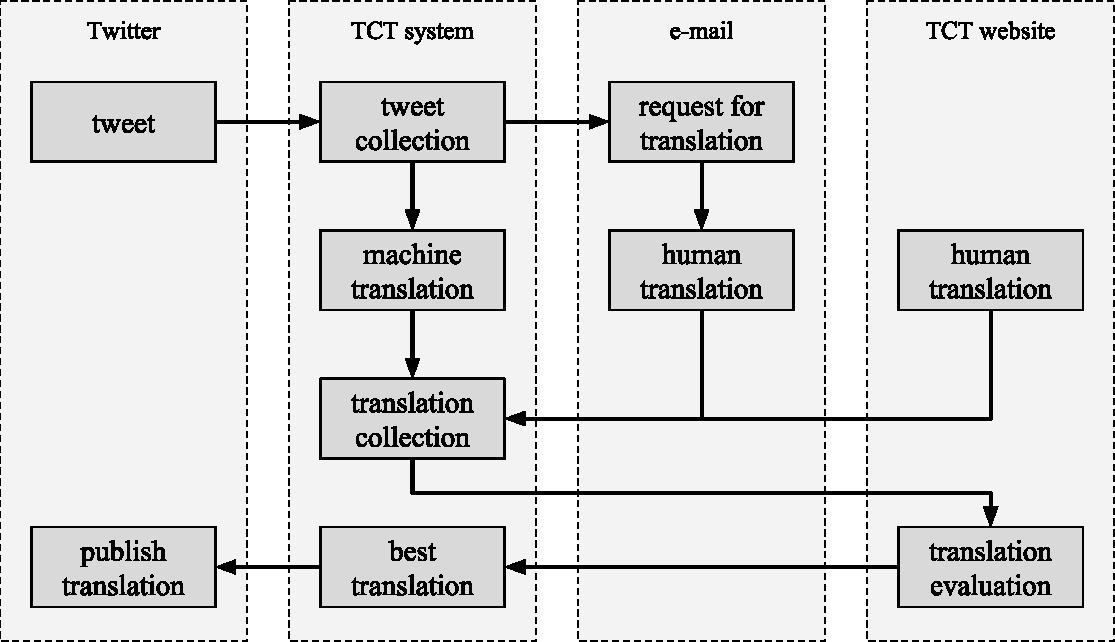
\includegraphics[width=\textwidth]{diagram}
		\end{figure}
	\end{center}
\end{frame}

% In case you would not know this is an example of a tweet. The interesting parts are the text of the tweet and also even though it is not visible here Twitter 
% automatically recognizes the language of the tweet.
% So far we manually select Twitter profiles to follow and collect tweets from. For example now we translate handful of sources from Ukraine to provide up to date information.
% In the future we plan to follow place specific tweets or follow a hashtag for a period of time to translate for example live events.
\setbeamercolor{background canvas}{bg=TCTwhite}
\setbeamercolor{normal text}{fg = TCTsilver}
\setbeamercolor{frametitle}{fg = TCTgray}
\begin{frame}
	\frametitle{Tweet Example}
	\begin{center}
		\begin{figure}
			
\includegraphics[width=\textwidth]{tweet01}
		\end{figure}
	\end{center}
\end{frame}

% Once the tweet enters TCT system it is sent out by mail to capable translators. They if interested provide their translation simply as a reply.
\setbeamercolor{background canvas}{bg=TCTwhite}
\setbeamercolor{normal text}{fg = TCTsilver}
\setbeamercolor{frametitle}{fg = TCTgray}
\begin{frame}
	\frametitle{TCT Workflow}
	\begin{center}
		\begin{figure}
			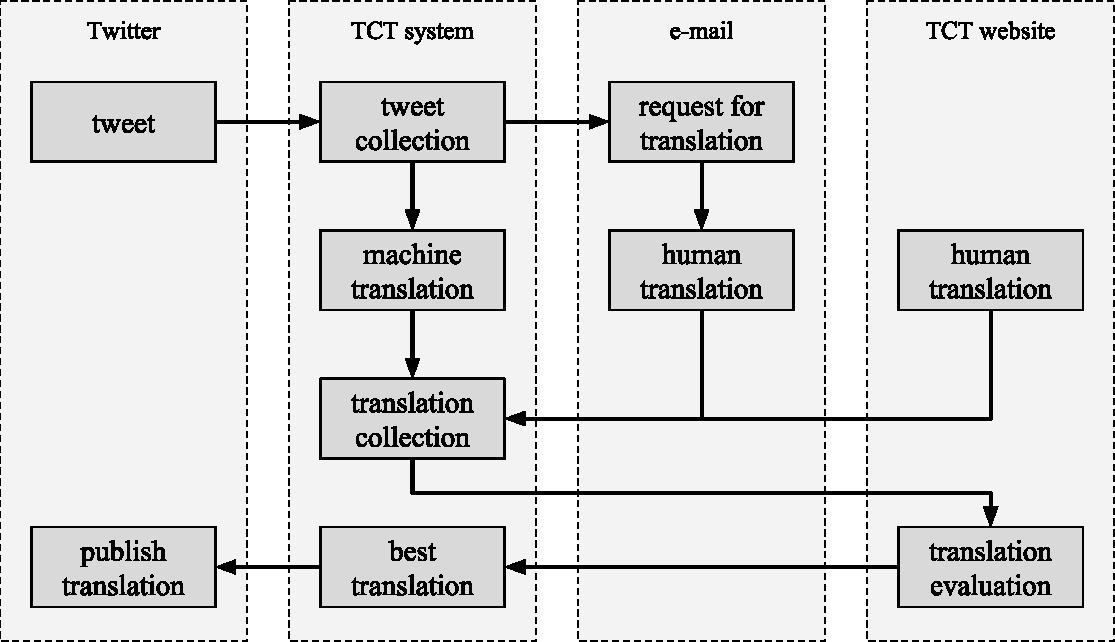
\includegraphics[width=\textwidth]{diagram}
		\end{figure}
	\end{center}
\end{frame}

% Here is an example of the request for translation sent to translators. It says the target language on the top and the original tweet bellow. 
% And under that is a hash to help us identify replies.
\setbeamercolor{background canvas}{bg=TCTwhite}
\setbeamercolor{normal text}{fg = TCTsilver}
\setbeamercolor{frametitle}{fg = TCTgray}
\begin{frame}
	\frametitle{E-mail Example}
	Please translate the following post to language: Czech
	\\[1cm]
	Practical overview of EU financial help to \#Ukraine - how much we provide, for what \& under what conditions;read here: bit.ly/1utqdbf
	\\[1cm]
	ID:51d46e56c720c0a20e98e7e628b5806a
\end{frame}

% Coming back to the diagram we see there is also an option to provide translation through TCT website. This was a request from our beta testers. 
% They wanted a way to submit a translation while browsing tweets in the database.
% And to see the potential improvement we also let the Moses MT translate each tweet.
% Everything meets again here at translation collection and from there we need to evaluate the best available translation. 
\setbeamercolor{background canvas}{bg=TCTwhite}
\setbeamercolor{normal text}{fg = TCTsilver}
\setbeamercolor{frametitle}{fg = TCTgray}
\begin{frame}
	\frametitle{TCT Workflow}
	\begin{center}
		\begin{figure}
			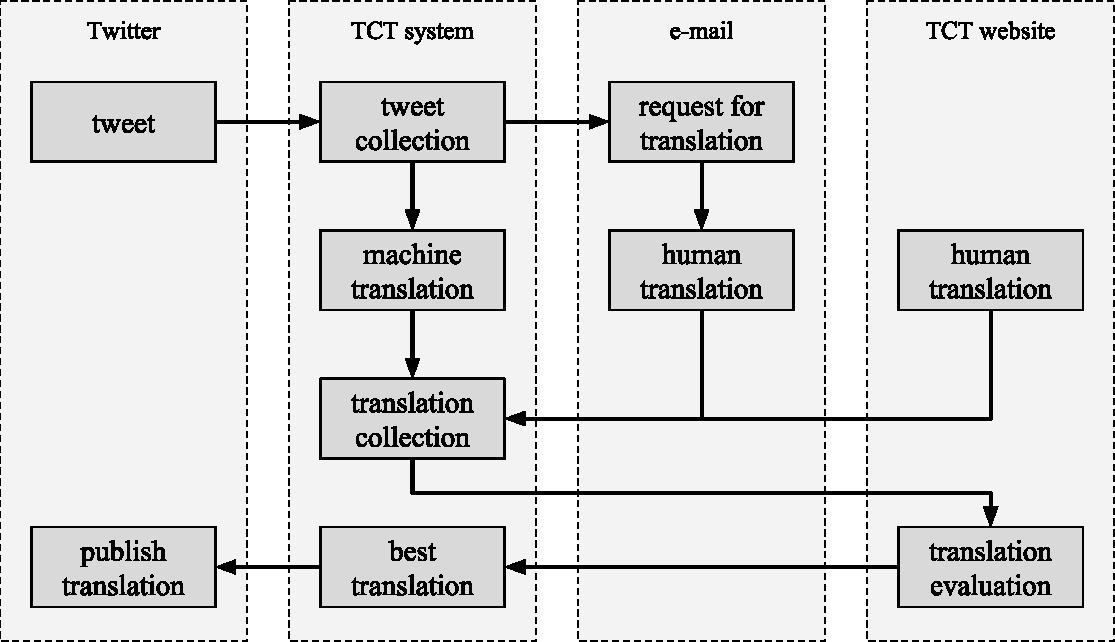
\includegraphics[width=\textwidth]{diagram}
		\end{figure}
	\end{center}
\end{frame}

% As of now the only way to evaluate translations is to visit our website. It is the only step in the process that requires user to do so.
% The evaluation is very basic. User is presented with a tweet one translation and is asked to select what best describes their attitude towards the translation.
% Options are "love it", "like it", "it's OK", "dislike it", "hate it" and "skip". By choosing these phrases instead of numbers or stars we hope to solve the 
% question "how much is a one star?"
\setbeamercolor{background canvas}{bg=TCTwhite}
\setbeamercolor{normal text}{fg = TCTsilver}
\setbeamercolor{frametitle}{fg = TCTgray}
\begin{frame}
	\frametitle{Translation Evaluation}
	\begin{center}
		\begin{figure}
			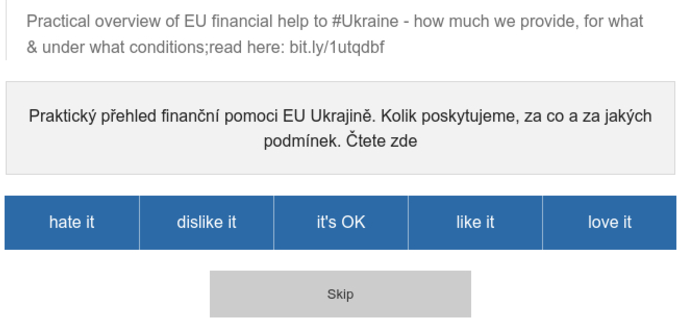
\includegraphics[width=\textwidth]{score}
		\end{figure}
	\end{center}	
\end{frame}

% And lastly we publish the best translation back to twitter.
\setbeamercolor{background canvas}{bg=TCTwhite}
\setbeamercolor{normal text}{fg = TCTsilver}
\setbeamercolor{frametitle}{fg = TCTgray}
\begin{frame}
	\frametitle{TCT Workflow}
	\begin{center}
		\begin{figure}
			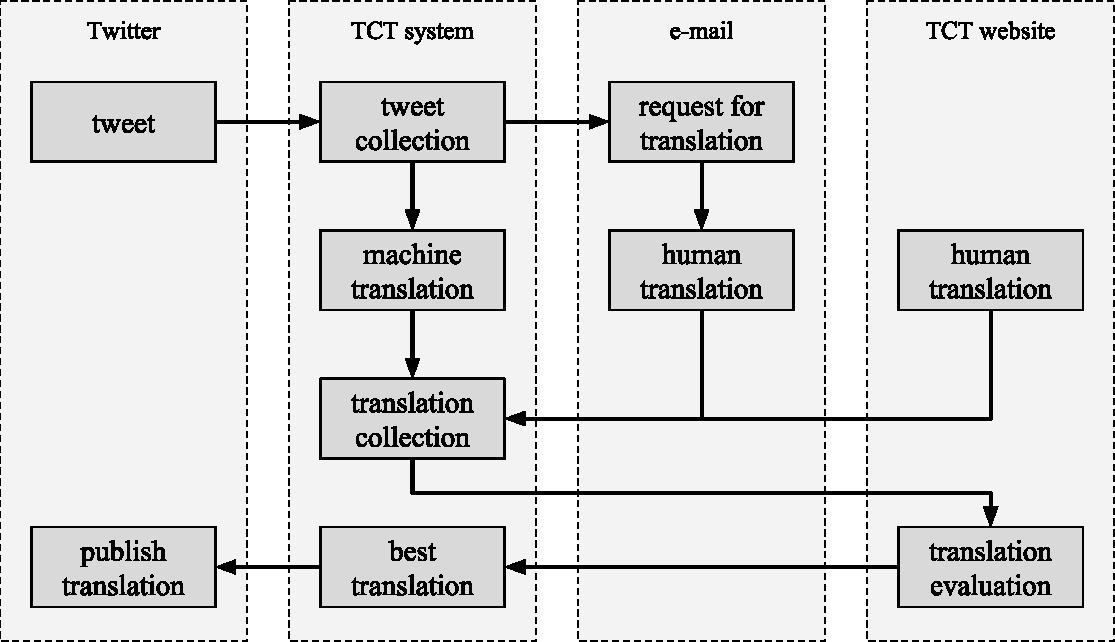
\includegraphics[width=\textwidth]{diagram}
		\end{figure}
	\end{center}
\end{frame}

% Since the TCT retweets the tweet before and then reply with our translation this is how the end user should see product of our work.
% I would like to point out that to get the translation user of Twitter only needs to follow our profile, nothing more outside or inside Twitter.
\setbeamercolor{background canvas}{bg=TCTwhite}
\setbeamercolor{normal text}{fg = TCTsilver}
\setbeamercolor{frametitle}{fg = TCTgray}
\begin{frame}
	\frametitle{Best Translation Published}
	\begin{center}
		\begin{figure}
			
\includegraphics[width=\textwidth]{tweet02}
		\end{figure}
	\end{center}	
\end{frame}

% The system as I have just described it is running in it's beta version on the following address. We are hopefully soon moving to more human friendly address but for now you can find us here.
% If we have time at the end I will gladly do a live demo but now I would like to talk about peculiarities of tweet translation we have discovered.
\setbeamercolor{background canvas}{bg=TCTblue}
\setbeamercolor{normal text}{fg = TCTsilver}
\setbeamercolor{frametitle}{fg = TCTwhite}
\begin{frame}
	\vfill
	\begin{center}
		\begin{figure}
			
\includegraphics[width=\textwidth]{TCT}
		\end{figure}
	\end{center}	
	\vfill
\end{frame}

% Unlike most other media the tweets are too short too carry sufficient context. With frequent abbreviations and misspellings they may even be difficult to understand for humans.
% Let's have a look at an example
\setbeamercolor{background canvas}{bg=TCTblue}
\setbeamercolor{normal text}{fg = TCTsilver}
\setbeamercolor{frametitle}{fg = TCTwhite}
\begin{frame}
	\frametitle{Tweet Translation Difficulties}
	\begin{itemize}
		\item \textcolor{TCTsilver}{\Large context}
		\item \textcolor{TCTsilver}{\Large abbreviations}
	\end{itemize}
\end{frame}

% Here are two tweets that we collected during the Ukraine situation and that alone is a missing context that may help you translate the abbreviations MRL and APC
% they are military vehicles by the way
% based on these observations we are in the process of implementing a context dictionary that could accompany the translation requests if translator would so desire

%but this issue gets even worse if you consider a picture or a video
%accompanying a tweet
% OB: ano, dalo se rict "a picture- or video-accompanied tweet", ale je to
% krkolomne
\setbeamercolor{background canvas}{bg=TCTwhite}
\setbeamercolor{normal text}{fg = TCTsilver}
\setbeamercolor{frametitle}{fg = TCTgray}
\begin{frame}
	\begin{center}
		Terrorists used \#Russian-supplied Smerch \alert<2>{MRL}s against \#Ukaine forces in th conflict zone http://t.co/s9ZKP2zsVk EMPR http://t.co/9ElqFP7qlg
		\\[0.7cm]
		Mykolaiv armored plant handed over 10 \alert<2>{APC}S  to the border guards  http://t.co/ANOtAKcUdw via $@$HromadskeTV http://t.co/mUmfbYKuwf
	\end{center}
	\uncover<2-> {\alert<2>{MRL} = multiple rocket launcher\\
	\alert<2>{APC} = armoured personnel carrier}
\end{frame}

% Consider this tweet. To me it is not really understandable until I see the images that accompany the tweet
% These examples actually bring us to another issue with tweet translation
\setbeamercolor{background canvas}{bg=TCTwhite}
\setbeamercolor{normal text}{fg = TCTsilver}
\setbeamercolor{frametitle}{fg = TCTgray}
\begin{frame}
	\begin{center}
	Russian SOF in Ukraine with "Polite People" \alert<2>{patch} and new \alert<2>{gear} \#CrisisUcrania http://t.co/gqLvuehCof
	\end{center}
	\uncover<2->{
		\begin{columns}
			\begin{column}{.5\textwidth}
				\begin{figure}
					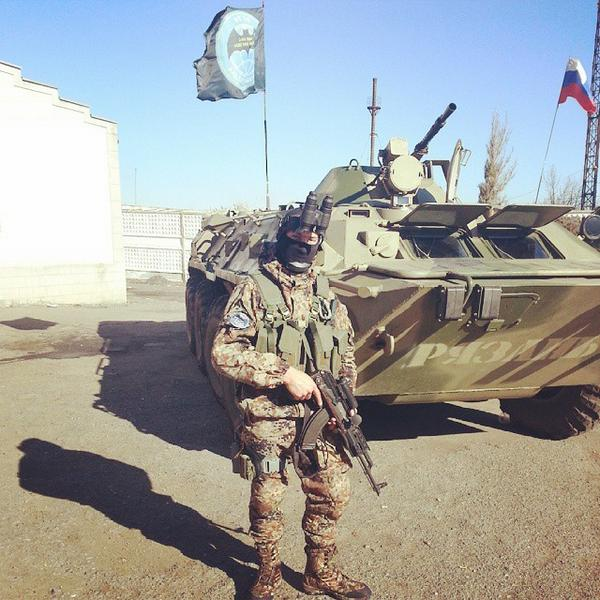
\includegraphics[width=\textwidth]{gear}
				\end{figure}
			\end{column}
			\begin{column}{.5\textwidth}
				\begin{figure}
					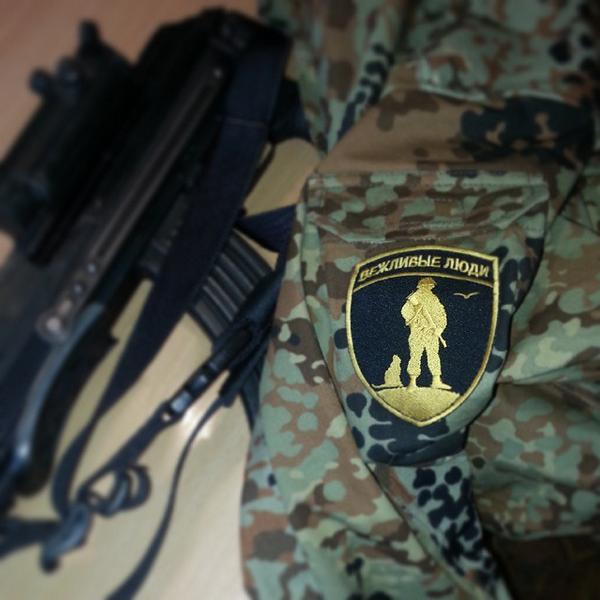
\includegraphics[width=\textwidth]{patch}
				\end{figure}
			\end{column}
		\end{columns}
	}
\end{frame}

% As you can see in previous examples tweets are often heavy on hashtags, URLs ang other user mentions. There are no guidelines on how to translate these
% Sometimes they are presented as a part of text and you immediately run in issues with declension.
% To make a long story short we have barely touched a tip of the iceberg and there is still tremendous amount of work to do.
% OB: na tomhle slidu by cast toho Tveho sdeleni mela byt napsana, ne? Nebo
% aspon zvyraznit ty hashtagy (jeden ma preklep i v originale) a pridat titulek,
% ze neni jasne, jak to prekladat.
\setbeamercolor{background canvas}{bg=TCTwhite}
\setbeamercolor{normal text}{fg = TCTsilver}
\setbeamercolor{frametitle}{fg = TCTgray}
\begin{frame}
	\begin{center}
		Terrorists used \#Russian-supplied Smerch MRLs against \#Ukaine forces in th conflict zone http://t.co/s9ZKP2zsVk EMPR http://t.co/9ElqFP7qlg
		\\[0.7cm]
		Mykolaiv armored plant handed over 10 APCS  to the border guards  http://t.co/ANOtAKcUdw via $@$HromadskeTV http://t.co/mUmfbYKuwf
	\end{center}
\end{frame}

\setbeamercolor{background canvas}{bg=TCTblue}
\setbeamercolor{normal text}{fg = TCTsilver}
\setbeamercolor{frametitle}{fg = TCTwhite}
\begin{frame}
	\frametitle{Summary}
	\begin{itemize}
		\item \textcolor{TCTwhite}{\Large device for human translation of tweets}
		\item \textcolor{TCTwhite}{\Large translation evaluation}
		\item \textcolor{TCTwhite}{\Large parallel corpus as a goal}
		\item \textcolor{TCTwhite}{\Large difficulties of tweet understanding}
	\end{itemize}
\end{frame}

% If you are now intrigued to find out more about our project you can first check the running beta if you are interested in the code it is available on GitHub
% We also have semi-updated blog and you can of course reach us on twitter
\setbeamercolor{background canvas}{bg=TCTblue}
\setbeamercolor{normal text}{fg = TCTsilver}
\setbeamercolor{frametitle}{fg = TCTwhite}
\begin{frame}
	\begin{center}
		\textcolor{TCTsilver}{\Huge Join us!}
		\\[0.9cm]
		\textcolor{TCTsilver}{\Huge quest.ms.mff.cuni.cz/tweeslate}
		\\[0.3cm]
		\textcolor{TCTsilver}{\Huge github.com/cifkao/tct }
		\\[0.3cm]
		\textcolor{TCTsilver}{\Huge tctranslation.blogspot.cz}
		\\[0.3cm]
		\textcolor{TCTsilver}{\Huge $@$tctranslation}
	\end{center}
\end{frame}

\end{document}
